\documentclass[11pt,letterpaper]{article}
\usepackage[margin=1.02in,headheight=14pt,footskip=26pt]{geometry}
\usepackage{lmodern}
\usepackage[T1]{fontenc}
\usepackage{amsmath,amssymb,amsthm,mathtools}
\usepackage{array,booktabs,xcolor,fancyhdr}
\usepackage[expansion=false]{microtype}
\usepackage[hyphens]{url}
\usepackage[colorlinks=true,linkcolor=teal!50!black,urlcolor=teal!60!black,citecolor=teal!50!black,pdfauthor={OpenAI},pdftitle={Finite presentations and cyclic proof replay in iPRA}]{hyperref}
\usepackage{titlesec,tikz}
\definecolor{ink}{HTML}{19374A}\definecolor{accent}{HTML}{237062}
\titleformat{\section}{\Large\bfseries\color{ink}}{\thesection}{.65em}{}
\titleformat{\subsection}{\large\bfseries\color{ink}}{\thesubsection}{.65em}{}
\setlength{\emergencystretch}{2.2em}
\setcounter{tocdepth}{1}
\renewcommand{\labelitemi}{\(\bullet\)}
\newtheorem{thm}{Theorem}[section]
\newtheorem{lem}[thm]{Lemma}
\newtheorem{prop}[thm]{Proposition}
\newcommand{\N}{\mathbb N}
\newcommand{\Q}{\mathbb Q}
\newcommand{\ipra}{\ensuremath{\mathsf{iPRA}}}
\newcommand{\cl}{\operatorname{cl}}
\newcommand{\bit}{\operatorname{bit}}
\newcommand{\repo}[2]{\href{https://github.com/VladimirReshetnikov/ProveIt/blob/3ee850b4c2d650cf01263823fd5415963747c5d0/Logic/PrimitiveRecursiveArithmetic/#1}{#2}}
\pagestyle{fancy}\fancyhf{}
\fancyhead[L]{\small\itshape Finite presentations and cyclic proof replay}
\fancyhead[R]{\small iPRA}\fancyfoot[C]{\small\thepage}
\renewcommand{\headrulewidth}{.3pt}
\raggedbottom
\begin{document}
\thispagestyle{plain}
\noindent{\color{accent}\sffamily\small PRIMITIVE RECURSIVE ARITHMETIC\hfill NOVEMBER 2026}\par
\vspace{1em}
\noindent{\huge\bfseries\color{ink} Finite presentations and cyclic\\[2pt] proof replay in iPRA\par}
\vspace{.55em}
\noindent{\large Category theory, topology, and local complex analysis\par}
\vspace{1em}
\noindent A finite observation of a mathematical object often has several proofs, each requiring different data. We give an arithmetic procedure which, for a finite table of positive rules, finds \emph{every inclusion-minimal set of external assumptions} sufficient for the observation. The rules can refer to each other cyclically. The procedure supplies ranks that turn successful searches into ordinary intuitionistic derivations. A converse on a simple path identifies exactly where a proposed uniform version would require stronger induction.

\medskip
\noindent The applications include sheafification on finite spaces, coherent lifts in inverse towers, and a decision procedure for rational polyhedral covers. For unions of closed rational boxes we give maps and homotopies to and from the intersection nerve. For the resonant Gauss equation we compute the coefficient that decides whether an independent local solution needs a logarithm, with explicit tail bounds through the second derivative.

\medskip
\noindent\textbf{Verification.} The archive contains six Lean modules and six exact-arithmetic programs. The replay module constructs ordinary iPRA proof objects. The application chapters pair human-readable arithmetic proofs with checked Lean lemmas and a path to complete object-language derivations.

\tableofcontents
\newpage
\section{What an embedding asserts}
\label{sec:scope}
We use the repository's ordinary first-order intuitionistic calculus with equality, numerical variables, one symbol for each primitive recursive (PR) definition, the successor axioms, and induction for quantifier-free formulas. A target written $\Gamma\vdash A$ means a derivation in that calculus. The repository implements it by \texttt{Prf PRAAx}. We used revision \texttt{3ee850b4c2d650cf01263823fd5415963747c5d0}. The distinction between archived proposals and integrated object derivations matters here. In particular, bounded-formula reflection, bounded rank induction, proof schedules and finite demand closure already have implementations. The FIBER audit still lists cyclic graph unrolling and application-specific producers as further work. Our cyclic result applies to finite positive rules, and the application sections identify specific producers. See the \repo{README.md}{repository overview}, \repo{Derivations/FIBER-CLAIMS.md}{FIBER audit} and \repo{Derivations/FINITE-DEMAND-CLAIMS.md}{finite-demand audit}.

\subsection{Objects, observations, and logic}
A presentation specifies numerical parameters $x$, a query $q$, a validity test or hypothesis $D(x)$, and the meaning $A(x,q)$ of a successful observation. For example $q$ may contain two morphism indices, a homological degree, a truncation order, or a precision. A finite proof of $A(x,q)$ may use auxiliary data $w$. One may publish $\exists w\,V(x,q,w)$, a specific PR witness $W(x,q)$ with $V(x,q,W)$, or a guarded implication. These are distinct claims. A proof using several approximations of a single object must establish that their restrictions or estimates agree.

A category with finitely many objects and arrows can be one numerical input with table laws. A tower with infinitely many levels instead has fixed PR symbols for enumeration and projection, with numerical parameters left free. A real number in the analytic interpretation is a specified PR sequence of rational approximations, with a proved error law. One may quantify over a finite table of rational samples, a clocked computation, or parameters to a fixed generator. A diagonal argument rules out a PR evaluator for all PR expressions. Given such an $E(e,n)$, $n\mapsto 1+E(n,n)$ would have an index $d$ with $E(d,d)=1+E(d,d)$. Thus a proof for each specified generator and a single arithmetical assertion about all its numerical inputs are entirely compatible. An unrestricted quantified assertion about all real functions or small categories needs a further interpretation.

We encode finite lists, products, signed integers and positive-denominator rational numbers by naturals. One concrete pairing is $2^a(2b+1)$, with $0$ reserved for the empty list. Decode its exponent-of-two valuation by search bounded by the code, then recover $b$ by division. Cons, length, lookup with defaults and all finite folds follow by PR operations (a decoder may run for the code as a clock). Numerals may grow very rapidly. We require a PR definition and a proof of its stated laws, with no polynomial running-time condition. Malformed inputs can return zero outside a displayed validity guard. A signed rational can use the parts $u-v$ and positive denominator $s+1$. Cross multiplication compares two such codes. An $\mathbb F_2$ vector uses a bit mask.

\paragraph{Induction convention.}
Fix the syntax of a bounded arithmetic formula $C$ whose bounds are PR terms, possibly depending on earlier variables. Equalities and orders have PR characteristic bits. Compute conjunction by multiplication, disjunction by maximum and negation by bit complementation. For decidable bits implication is tested by $\neg a\lor b$. A bounded universal is the product of its instances, a bounded existential their maximum, with empty values $1$ and $0$. For example, the product over $i<t$ is $1$ precisely if all $t$ factors are $1$. One direction follows by deriving the endpoint and prefix facts from the successor equation by induction on a bit statement, and instantiating at an arbitrary in-range index. Conversely from a supplied universal premise each next factor is $1$, so a QF induction gives product $1$. Bounded search gives the analogous witness for the maximum. Structural recursion in the metatheory establishes $C\leftrightarrow(\bit_C=1)$, including dependent bounds. We use this reflected equation whenever we induct on a finite array property. Quantified hypotheses can be held fixed in the context during QF induction. The repository's \repo{Derivations/Lean/IPRADerivations/Foundations/BoundedSyntaxInduction.lean}{bounded induction module} implements this convention.

\paragraph{Meaning of a finite-precision theorem.}
The internal content of an error bound for a series is a bound on \emph{every finite tail} beyond a given numerical cutoff. This yields compatible rational outputs with a PR modulus. Convergence or equality of functions in an ambient analytic model is the mathematical reading of these outputs. Likewise our nerve theorem gives matrices and identities, and sheafification gives compatible tuple codes and mutual inverses. Ordinary Lean proofs about mathematical structures help verify the interpretation. A Lean theorem whose conclusion is $\Gamma\vdash A$ supplies different evidence. Section~\ref{sec:replay-guide} records which kind is present for each result.


\paragraph{Equality and maps of names.}
For a rational metric presentation $(D,d)$ with PR distance, call $a$ regular when
$d(a_i,a_j)\le 2^{-i}+2^{-j}$ for all $i,j$, with all samples in $D$.
Use fixed PR sample programs with numerical parameters. Define $a\sim b$ by
$d(a_i,b_j)\le 2^{-i}+2^{-j}$ for every $i,j$. Regularity gives reflexivity, and symmetry follows from that of $d$. For transitivity insert the middle sample $b_t$ between $a_i$ and $c_j$. The bound becomes $2^{-i}+2^{-j}+2^{1-t}$. If the rational distance exceeded $2^{-i}+2^{-j}$ by $r/s>0$ with positive integers $r,s$, taking $t=s+2$ makes $2^{1-t}<1/s\le r/s$, a contradiction. Thus $\sim$ is an equivalence relation, proved at arbitrary fixed outer indices.

For an exactly evaluated rational Lipschitz map $f$ of bound $L$, take the least $h\le 1+\lceil L\rceil$ with $2^h\ge\max(1,L)$ and set $F(a)_p=f(a_{p+h})$. The input estimate multiplied by $L$ gives the output estimate at $p,q$, both for regularity and preservation of $\sim$. If the evaluator contributes error at most $2^{-(p+1)}$, use $p+h+1$ for the input and split the budget in half. Identity respects $\sim$, and composition adds the input shifts. Different safe shifts give equivalent outputs by the cross-index inequality above. In this way a quotient by equality of names can be used externally while each equality proof consists of rational inequalities inside arithmetic. This construction supplies the meaning of the maps on regular names in the box example.

\section{Cyclic rules, exact assumptions, and induction}
\label{sec:rules}
A query may have two producers, one geometric and one algebraic. Either producer may request other observations. Requiring every incoming assumption can lose a theorem. Accepting a loop because each member has a supporting rule can prove an arbitrary assertion from itself. The following finite procedure determines precisely which assumptions suffice \emph{using the specified rules}.

\subsection{Arithmetic evaluation of a finite rule table}
A table has $N$ observation labels and $b$ external ports, all numbered from zero. Each row $e=(h,P,G)$ has a head $h<N$, a set $P$ of prerequisite labels and a set $G$ of required ports. The intended inference derives $h$ from all of $P$ and all of $G$. Multiple rows can have the same head. Supply a set $S$ of ports. Masks code all these sets. Define, by numerical recursion,
\[
 X_0=0,\qquad
 X_{k+1}=X_k\cup
 \{h:\text{some row }(h,P,G)\text{ has }P\subseteq X_k,\ G\subseteq S\}.
\]
In this display $0$ is the empty mask and all searches run through the table. Write $C(S)=X_N$. A rule with empty prerequisite set can enter in round one. A head without rules never enters.

\begin{thm}[Finite replay and its converse certificate]\label{th:closure}
$C(S)$ is the least set closed under the enabled rules. A label belongs to it exactly when it has a finite tree of applications with supplied ports. On success the algorithm returns the first-entry rank and a justifying row at every marked label. On failure it returns a closed subset omitting the requested label. Both types of evidence are checkable primitive recursively.
\end{thm}
\begin{proof}
An increase marks at least one previously unmarked label. The count of marked bits is bounded by $N$. Equality of two consecutive masks implies equality of the successors because the update is deterministic. Induction gives the alternative $|X_k|\ge k$ or $X_k=X_{k+1}$. At $k=N$ another increase is impossible. In fact the number of distinct heads suffices. If $T$ is any closed mask, induction on the bit $[X_k\subseteq T]$ puts every stage inside $T$. These arguments allow the entire table to be an internal variable.

For a newly marked head store the first eligible row in the table. Every child has smaller first-entry rank. Following those choices produces a finite proof tree with branch length at most $N$ (the shared table of choices usually uses less space). Conversely, leaves with empty prerequisite sets enter immediately, and if all child trees have height at most $j$ their parent enters by stage $j+1$. A coded tree can be verified instead as a list in children-first order. Induct on the Boolean claim that every checked entry in the prefix has its label in the closed mask $C(S)$. Thus no uniform recursion on arbitrary tree objects is needed. A positive certificate only needs a marked fragment containing the root, enabled justifications, and strictly descending natural ranks. A closed mask $T$ with $v\notin T$ certifies failure by leastness. For a certificate of the complete output, check both conditions on the same mask. The empty graph, empty supply and a self-supporting isolated cycle all obey these tests.
\end{proof}

The operation is monotone in $S$, by induction on the inclusion of the two masks obtained with smaller and larger supplies. Define
\[
 {\cal M}_v=\{S<2^b:v\in C(S),\
       \forall p\in S,\ v\notin C(S\setminus\{p\})\}.
\]
For finite sets of bits we identify a set with its code. A supply $T$ works if and only if it contains some $S\in{\cal M}_v$. Starting from successful $T$, scan its ports, removing one whenever the smaller set still succeeds. A removal that fails cannot become successful after further deletions, by monotonicity. The scan produces the required $S$. This proves the equivalence by bounded tests and yields all minimal alternatives by enumeration. An empty family expresses impossibility by these rules. A family containing $\varnothing$ expresses an unconditional route. Distinct sets can transmit logically equivalent assumptions in a mathematical interpretation, so minimality here is a property of the table.

For example take two labels $u,v$, the rules $u\leftarrow v$, $v\leftarrow u$, and two entry rules $u\leftarrow p,q$, $v\leftarrow r$, where $p,q,r$ are ports. The minimal supplies for $u$ are $\{p,q\}$ and $\{r\}$. When only $p$ is available the empty closed mask witnesses failure. When $r$ is available the certificate enters $v$ in round one and $u$ in round two. Treating the strongly connected pair as already proved would erase both genuine conditions.

\subsection{Composition across a finite interface}
Partition the labels into $U,V$. Write $F(X,Y)$ and $G(X,Y)$ for the monotone one-round consequence operators on the respective coordinates, including retention of their own bits, with $S$ fixed. Let $y(X)$ be the least closed $Y$ for $Y\mapsto G(X,Y)$, found in at most $|V|$ rounds starting empty. Compute $x_*$ by iterating $X\mapsto F(X,y(X))$ from empty for $|U|$ rounds. Then the joint result is $(x_*,y(x_*))$.

Indeed $X\subseteq X'$ implies $y(X)\subseteq y(X')$ by iteration, so the outer loop is monotone and inflationary. Both equations hold at the proposed result. For any jointly closed $(A,B)$ one has $y(A)\subseteq B$, then $F(A,y(A))\subseteq A$. Outer leastness gives $x_*\subseteq A$ and inner monotonicity gives $y(x_*)\subseteq B$. All comparisons are mask inclusions. Equivalently precompute each inner output's minimal supports among the outer input labels and original ports, then substitute these disjunctive summaries into the outer rules. For fixed supplies they compute exactly $y(X)$ by the preceding result. This finite version of Beki\'c elimination permits replacing a module even when its outputs feed back into its inputs. Only positive use of these labels is allowed. Positive-rule saturation and alternative explanations also have a long history in deductive databases \cite{green}. Here the two replay judgements identify the induction needed for the iPRA interpretation.

\subsection{From labels to arithmetic derivations}
Fix externally a finite table. Assign an arbitrary object formula $A_v(\vec x)$ to each label and $R_p(\vec x)$ to each port. Supply, for every row, an actual local derivation
\[
 (A_i)_{i\in P},\ (R_j)_{j\in G},\ \Gamma\ \vdash A_h .
\]
The variables $\vec x$ stay free. From derivations of the supplied $R_j$ in $\Gamma$, replay in increasing rank. At a marked row, simultaneous cut substitutes the already constructed proofs of its prerequisites and the designated port proofs. This gives $\Gamma\vdash A_v$. A minimal supply $S$ therefore gives a derivation from $\Gamma,(R_j)_{j\in S}$. Intuitionistic disjunction elimination yields
\[
 \Gamma\vdash
 \left(\bigvee_{S\in{\cal M}_v}\ \bigwedge_{p\in S}R_p\right)
       \longrightarrow A_v ,
\]
with the usual empty disjunction $\bot$ and empty conjunction $0=0$. No decision procedure for $R_p$ was used. The operations on masks concerned the availability of proofs. In a context with a local existential witness the row is replayed under that fresh variable. Existential elimination then applies if the public conclusion and the outside context do not depend on it. Supplying a port globally from different local choices requires its own derivation.

\paragraph{An internal number of stages.}
For a numerical input table and a fixed formula family $A(x,v)$, assume it has a reflected bounded matrix for the observations being propagated, and that the local rule and port implications have uniform object proofs. In the theory fix $x,S$ and retain the port and row hypotheses in context. Use the single bit
\[
 I(k)=\Big[\forall v<N\ (v\in X_k\ \longrightarrow A(x,v))\Big].
\]
The zero case is the empty mask. For a newly marked label select a row by bounded search, apply $I(k)$ to its finite prerequisites, then use its rule. This gives the next reflected bit. QF induction gives $I(N)$ at the input size. A more general public conclusion $B(x,v)$ is available if there is a proved exit implication from the bounded invariant to $B$. For example, an algorithm may store its chosen witnesses in a table. Its invariant asserts by bounded tests that each stored witness verifies its label. At entry, run a specified PR constructor on the previous table and append the result. A bound on the \emph{output} witness can be derived if needed by maximizing each fixed constructor over inputs bounded by the current code bound, then iterating the maximum for $N$ rounds. Existential introduction at exit exports the stored witness. An unspecified witness source remains a premise. For bounded labels the internal arithmetic proofs here are on paper. The supplied Lean module already implements the external derivation family for arbitrary labels.

\begin{prop}[Strength of uniform path replay]\label{p:path}
For any class of formulas closed under substitution of numerical terms and addition of parameters, uniform replay along the paths $0,1,\ldots,n$ for that class is equivalent over iPRA to its induction schema. With a global step hypothesis the equivalence also holds for each single formula.
\end{prop}
\begin{proof}
Use the exact path principle
\[
 \forall n\ \bigl(A(0)\land \forall i<n\,[A(i)\to A(i+1)]
                  \ \longrightarrow A(n)\bigr).
\]
Assume it, a base, and unrestricted local progress. Restrict progress to $i<n$ for arbitrary $n$ and apply the displayed principle. Conversely assume the induction schema for the class. Derive the bounded path assertion using induction on the \emph{clamped instance} $A(\min(i,n),\vec x)$. At $i<n$ apply the given step and otherwise use equality of consecutive clamped indices. Instantiate at $n$. The clamped formula belongs to the class by its substitution hypothesis. Replacing the bounded step by a global premise removes the closure requirement. The resulting principle with premise $\forall i\,[A(i)\to A(i+1)]$ is intuitionistically equivalent, by quantifier rules alone, to the single induction axiom for $A$. Thus allowing arbitrary formulas in the input-length replay rule recovers full first-order induction. The checked replay theorem for fixed finite tables avoids this increase in strength.
\end{proof}

\section{Computing a missing cover margin}
\label{sec:atlas}
A continuous argument often calls a local procedure after choosing a chart containing the point and a neighborhood around it. An effective lower margin allows that chart to be chosen from an approximation. The \repo{Derivations/Lean/IPRADerivations/Foundations/MeshPositivity.lean}{mesh-positivity proof} transfers a supplied positive grid estimate. For finite unions of rational polyhedral charts we can compute the \emph{best} lower slack directly. Its size depends on the chosen inequality presentation.

Let $D=[0,1]^d$. Chart $i$ has a nonempty list of affine forms $\ell_{ij}\in\Q[x_1,\ldots,x_d]$ and accepts a point when all its forms are strictly positive there. Assume at least one chart. Put
\[
 f_i(x)=\min_j\ell_{ij}(x),\qquad f(x)=\max_i f_i(x).
\]
The minimum in the following theorem comes with both a rational value and a rational point of attainment. The internal comparison quantifies over rational codes for $x$.

\begin{thm}[Sharp rational chart margin]\label{th:atlas}
Uniformly in $d$ and in the input tables there are PR outputs $x_0\in D\cap\Q^d$ and $\mu=f(x_0)$ such that every rational $x\in D$ satisfies $f(x)\ge\mu$. The union covers the cube with strict charts exactly when $\mu>0$. In the positive case it also covers regular Cauchy names with a uniform neighborhood radius on which a selected chart works.
\end{thm}
\begin{proof}
Make a list of the $2d$ coordinate face planes and every equality plane $\ell=\ell'$ between input atoms. A constant or zero equation is allowed in the list and can never participate in an independent system of $d$ rows when $d>0$. For every $d$-element sublist, use the determinant to test independence, solve by Cramer's rule, discard solutions outside $D$, and retain the surviving point with least $f$. The cube corners occur and $d=0$ uses the zero-by-zero determinant $1$ and the empty tuple. Every operation is a bounded scan. We show that the list is sufficient without invoking compactness for arbitrary continuous functions.

Take any rational $x\in D$. Sort all atoms by their values at $x$, breaking ties by index. Intersect the cube with the weak inequalities that impose this ordering. On the resulting bounded rational polyhedron $P$, $f$ is one fixed atom $\ell$ because taking the minimum in each group and then the maximum simply selects its position in the order. At $x$, collect the normals of the tight inequalities, including all tight coordinate faces, of rank $r$. If $r=d$, independent tight equations already identify a listed point. If $r<d$, Gaussian elimination gives a rational nonzero vector $v$ annihilated by all these normals. Reverse its sign if needed so that the slope of $\ell$ along it is nonpositive. For each inequality written $a\cdot y\le b$ with $a\cdot v>0$ compute $(b-a\cdot x)/(a\cdot v)$. There is at least one such constraint because the box contains both coordinate faces for each nonzero component of $v$. Each ratio is positive, as tight constraints have zero slope. Move by the smallest of these ratios. The new point is rational, obeys all inequalities, retains every tight equality, and has $f$ no larger than before. The new tight normal with positive pairing against $v$ raises the rank. After at most $d$ moves there is a listed point with $f\le f(x)$. This proves the rational assertion, including lower-dimensional ordering cells and ties.

For each atom let its slope bound be the sum of the absolute values of its linear coefficients, and let $L$ be their maximum. The functions $f_i,f$ are $L$-Lipschitz for the sup norm, since a maximum or minimum of a finite list changes by at most its largest component change. If $\mu\le0$, the rational output $x_0$ fails every strict chart. If $\mu>0$, define $\delta=\mu/(4\max(1,L))$. Given a name in $D$, choose a rational $q\in D$ with error at most $\delta$ by a dyadic precision request and coordinatewise clipping. Choose a maximizing chart for $f(q)$ by rational comparisons. At every point of $D$ within $\delta$ of the named point that same chart has slack at least $\mu-2L\delta\ge\mu/2$. In the arithmetic reading the last statement means the corresponding rational estimates at all requested precisions. Thus one can decide coverage on the supplied finite class and produce a working neighborhood, even when the original specification declared only pointwise positivity.
\end{proof}

\paragraph{Sizes and induction.}
Clear the denominators of \emph{all} affine forms with a common positive multiplier $D_0$. Let $B\ge1$ bound in absolute value every integer coefficient of the resulting arrangement equations, including constants and face equations. The determinants in the enumeration have absolute value at most $d!B^d$ by the permutation formula. Each candidate value of $f$ has a denominator at most $D_0d!B^d$ in lowest terms. In particular, positive $\mu$ has the explicit lower bound $1/(D_0d!B^d)$. The rank computation can scan square minors of size at most $d$. Solving a nonsingular maximal minor with one unmatched coordinate set to one and the other free coordinates zero gives the required null vector. Maximality makes it annihilate the remaining rows as well. To internalize the descent, fix the rational $x$ in the context, run exactly $d$ steps with full-rank states held fixed, and induct on the bounded tests for membership, nonincrease of $\ell$, and $\mathrm{rank}\ge\min(k,d)$. The arithmetic behind Cramer's rule follows by expanding the determinant multilinearly in a column. Every expansion with two equal columns cancels by interchanging them. Rank can equivalently be tracked by elimination with pivot search guarded by a nonzero numerator, an operation on finite tables of rational codes.

\paragraph{Two examples.}
Define four charts of the square by choosing independently between $x<2/3$ or $x>1/3$, and $y<2/3$ or $y>1/3$. With slacks $2/3-x,x-1/3$ and their $y$ analogues, the best common margin is $1/6$, attained for example at $(0,1/2)$. The arrangement includes the tie planes, while testing the original four vertices would yield $2/3$.

For analytic continuation, consider the segment $z(t)=t+i(2t-1)$, $0\le t\le1$, and punctures $0,1$. Each $\|z(t)-a\|_\infty$ is the maximum of four signed affine coordinates. The clearance to the pair is the minimum of two such maxima. Distributing $\min(\max_i u_i,\max_j v_j)=\max_{i,j}\min(u_i,v_j)$ puts it in the required format. Its exact minimum is $1/3$ at $t=1/3,2/3$. This supplies a singularity-clearance input for a path continuation routine. Other inputs, for instance the growth of solutions along the path, require separate arguments. A polygonal path and a finite list of rational punctures work by the same finite distribution and a minimum over segments. The accompanying \path{code/atlas.py} implements the determinant enumeration.

\section{Two categorical constructions with finite witnesses}
\label{sec:categorycases}

The repository's categorical packet constructs finite limits and glues
ordinary function tables on a finite cover. Its object-calculus development
also derives coherent points for towers with bounded surjective lifting.
We construct the sheaf associated to a supplied presheaf and extract the part of an inverse tower on which lifting works.
Background on finite-space sheaves and stabilization appears in \href{https://arxiv.org/abs/math/0610685}{Ladkani, \S2.2}, and the
\href{https://stacks.math.columbia.edu/tag/0594}{Stacks Project, Tag 0594}. See also the \repo{docs/proofs/foundations/ipra_categorical_methods/paper/sections/05_descent.tex}{ProveIt descent packet}.

\subsection{Sheafification on an arbitrary finite topological space}

Fix a topology on $X=[d]=\{0,\ldots,d-1\}$. Encode an open by its
$d$-bit mask, and the topology by its table on $2^d$ masks.
Require the empty and full masks to be open and check binary unions and
intersections. These suffice because there are finitely many masks.
A finite presheaf $F$ is a number $f_U$ for each open, with
$F(U)=[f_U]$, and a restriction table $r^F_{UV}:F(U)\to F(V)$
for each open $V\subseteq U$. Test identity and composition entrywise.
A morphism of presheaves is a family of tables commuting with restrictions.
A sheaf $G$ is required to pass a finite gluing test. For every cover of $U$
and every family of sections agreeing on pairwise intersections, there is
exactly one section in $G(U)$ restricting to that family. A cover is
a subfamily of the topology whose union is $U$. Removing repeated masks
causes no loss, since matching sections on repeated patches are equal.
This includes the empty cover of the empty open.

For $x\in X$, let $N_x$ be the intersection of all opens containing $x$.
It is open, contains $x$, and is contained in any open containing $x$.
In particular $y\in N_x$ implies $N_y\subseteq N_x$.
For an open $U$, define $SF(U)$ to be the compatible tuples
\[
 (a_x)_{x\in U},\qquad a_x\in F(N_x),\qquad
 r^F_{N_xN_y}(a_x)=a_y\quad(x\in U,\ y\in N_x).
\]
Order all tuples lexicographically and code a compatible tuple by its rank
in the retained list. For the empty open there is one tuple.
Restrict by deleting coordinates. On a morphism $h:F\to G$, apply
$h_{N_x}$ coordinatewise. Naturality of $h$ proves compatibility.
Identity and composition follow by evaluating at each coordinate. Define
$\eta_{F,U}(t)_x=r^F_{UN_x}(t)$. The presheaf identities prove that these
tuples are compatible, natural in $U$, and natural in $F$.

\paragraph{Theorem.}
$S$ is a uniform PR sheafification for finite-set-valued presheaves on
finite spaces. Composition with $\eta_F$ gives a PR bijection
\[
 \operatorname{Hom}_{\rm Sh}(SF,G)\ \longrightarrow \operatorname{Hom}_{\rm PSh}(F,G)
\]
for every supplied finite sheaf $G$. Both inverse equations have
finite arithmetic proofs.

\paragraph{Proof.}
Take matching tuples on a cover of $U$. For each $x\in U$ read its
entry in the first patch containing $x$. Agreement on intersections
makes this independent of the patch. If $y\in N_x$, the chosen patch
containing $x$ also contains $y$, so compatibility of its tuple gives
the required restriction equation. These forced entries prove
existence and uniqueness of the glued tuple. It includes the empty cover.

Over $N_x$, evaluation at $x$ identifies $SF(N_x)$ with $F(N_x)$.
Indeed $b\in F(N_x)$ gives the tuple $y\mapsto r^F_{N_xN_y}(b)$
and compatibility forces every tuple on $N_x$ to have this form.

Given $h:F\to G$ and $a\in SF(U)$, form $g_x=h_{N_x}(a_x)$.
To glue $g_x$ and $g_z$ on $W=N_x\cap N_z$, take any $y\in W$.
Both restrict to $h_{N_y}(a_y)$ on $N_y$, by naturality and
compatibility. The opens $N_y$ cover $W$. Uniqueness in the sheaf
condition makes the two restrictions equal on $W$, including when
$W$ is empty. Thus the $g_x$ match. Define $\bar h_U(a)$ by scanning
$G(U)$ for their unique glue. Its restrictions to smaller opens
give the same answer by uniqueness on their minimal-neighborhood covers.
This proves naturality in $U$. For $t\in F(U)$ the required glue of the
components of $\eta_F(t)$ is $h_U(t)$, proving $\bar h\eta_F=h$.
Conversely, if $k\eta_F=h$, then on $N_x$ the bijection above forces
$k_{N_x}(a|_{N_x})=h_{N_x}(a_x)$. Naturality and uniqueness on
the cover of $U$ give $k_U(a)=\bar h_U(a)$. This proves the second
inverse equation. Compatibility with pre- and postcomposition follows since
the two candidate extensions have the same composite with the unit.
Taking $F$ itself to be a sheaf, its neighborhood sections glue uniquely,
so $\eta_F$ is an isomorphism. In particular $S(SF)\cong SF$.

\paragraph{Arithmetic bounds and example.}
With $q=2^d$ and $D=\max(1,\max_U f_U)$ (the maximum over opens),
there are at most $D^d$ candidate tuples over each open, including the
single empty tuple. If any required coordinate has an empty alphabet, reject the tuple before digit extraction. Mask scans have bound $q$, subfamily
scans $2^q$. If validating a sheaf with fiber bound $H\ge1$, cover
assignments number at most $H^q$, and the uniqueness scan has bound $H$.
Keep the tuple, prefix agreement bits, number of matches truncated at two,
and first matching index. Induct on their bounded prefix specifications.
All induced names, restrictions, unit and extension tables thus use only
PR loops, also when the input topology varies. For the discrete
two-point space, take the constant presheaf $F(U)=[2]$ with identity
restrictions, including at the empty open. Then $SF(X)$ has four sections,
$SF(\varnothing)$ has one, and $\eta_{F,X}$ sends $b$ to $(b,b)$.
This construction applies to spaces with smallest neighborhoods. An arbitrary infinite space may lack
smallest open neighborhoods.

\subsection{Stable images in an inverse tower}

Fix PR bounds $b_n$, Boolean membership predicates for
$A_n\subseteq[b_n]$, and PR bonding maps
$p_n:A_{n+1}\to A_n$ with proofs of typing.
For $m\ge n$ let $P_{n,m}:A_m\to A_n$ denote the composite, identity
when $m=n$. Starting with $z$ at $m$, iterate $j\mapsto
p_{m-1-j}$ on the register for $m-n$ steps.
Splitting this finite loop at any intermediate $k$ gives
$P_{n,k}P_{k,m}=P_{n,m}$. More explicitly, resume the run after
$m-k$ steps. Induction on the number of resumed steps gives identical
registers in both runs because both use the same next bond.
Let $I_{n,m}=P_{n,m}(A_m)$. Membership is one bounded search below $b_m$.
Images decrease as $m$ increases, by the composite law.

A proposed rate is a fixed PR $s(n)\ge n$. Set $B_n=I_{n,s(n)}$,
$K_n=\max(s(n),s(n+1))$. Consider the single comparison at each $n$
\begin{equation}
       I_{n,s(n)}\subseteq I_{n,K_n}.                   \tag{C}\label{eq:catcap}
\end{equation}
After fixing $n$ this is a bounded Boolean test, even though its validity
for every $n$ is a global arithmetic hypothesis. No monotonicity of $s$
is assumed.

\paragraph{Theorem.}
Condition \eqref{eq:catcap} at every $n$ is equivalent to
$I_{n,t}=B_n$ for all $n$ and $t\ge s(n)$.
From the former, a PR algorithm extends every given $a\in B_n$ to a
coherent sequence on all levels $n,n+1,\ldots$. The original bonding
maps may fail to be surjective.

\paragraph{Proof.}
If the images stabilize by $s(n)$, take $t=K_n$. Conversely, fix
$a\in B_n$. Condition \eqref{eq:catcap} yields a successful search
for $z\in A_{K_n}$ with $P_{n,K_n}(z)=a$. Put
$c=P_{n+1,K_n}(z)$. Projecting $z$ first to $s(n+1)$ shows that
$c\in B_{n+1}$, and $p_n(c)=a$ by the composite law.
Thus bounded search constructs a PR successor $L(n,a)$ with a
default value on invalid input. Define $w(0)=a$ and
$w(j+1)=L(n+j,w(j))$. At every $j$,
\[
     w(j)\in B_{n+j}, \qquad P_{n,n+j}(w(j))=a .
\]
Induct on the conjunction, compiling the first membership into its bounded
Boolean image test. The successor step is the lift just proved and one
composition of projections. In particular $p_{n+j}(w(j+1))=w(j)$.
For $t\ge s(n)$ choose $j=t-n$. Then $w(j)\in A_t$ supplies the missing
witness that $a\in I_{n,t}$. The reverse inclusion follows from decreasing
images. This proves the equivalence and exhibits the sequence as a
specified PR function of $n,a,j$. To see that $p_n(B_{n+1})\subseteq B_n$, apply the now proved stabilization at level $n+1$ and time $K_n$,
then project from $K_n$ to $s(n)$. The restricted tower is surjective.

\paragraph{Application to exactness.}
Let $q_n:G_n\to H_n$ be surjective homomorphisms of PR-presented
finite abelian groups, compatible with the bonds, and assume
\eqref{eq:catcap} with rate $s$ for the tower of kernels.
Every specified PR coherent $h_n\in H_n$ then has a PR coherent lift
$g_n\in G_n$. Indeed let $E_n=q_n^{-1}(h_n)$, a nonempty decidable fiber
with the inherited bonds. For $a\in I^E_{n,s(n)}$ take a preimage
$e\in E_{s(n)}$, and choose any $z\in E_{K_n}$ by bounded search.
The difference $e-P_{s(n),K_n}(z)$ lies in $\ker q_{s(n)}$.
Its image $a-P_{n,K_n}(z)$ at $n$ therefore lifts, by the kernel
comparison, to $d\in\ker q_{K_n}$. Now $z+d\in E_{K_n}$ projects to
$a$. This proves the comparison for $E$ with the very same rate.
Project any member of $E_{s(0)}$ to level zero for a seed, and apply the
walk just constructed. This gives an arithmetic, parameter-wise form of
exactness of the inverse limit at the right-hand term. All choices in
the argument are bounded scans.

For example, let every $A_n=\{0,1,2\}$ and every bond fix $0,1$ and
send $2$ to $1$. Then $s(n)=n+1$ works and $B_n=\{0,1\}$.
Even two elements per level permit towers for which no rate can be computed uniformly from a tower index.
For program $e$, let $A_0=\{0,1\}$. For $n>0$ use the same two elements
until bounded simulation by time $n$ reports a halt, then use only $0$.
The maps are inclusions. A uniform computable rate would decide halting since $1\in I_{0,s(0)}$ exactly when $e$ never halts, by stability and the
definition of the tower. This is an external impossibility result.
Every tower in this example already has the constant zero branch. The
information a rate recovers is extendibility of \emph{all} persistent
states, which is stronger than a single branch.

\paragraph{Lean endpoints.}
\path{lean/SheafCase.lean} proves the principal-cover gluing and both inverse equations in ordinary Lean, using the specialization preorder $x\preceq y$ iff $y\in N_x$. Its \texttt{SheafGluing} structure records the glue, its restrictions and uniqueness. The preceding proof constructs these operations from a finite sheaf table. \path{lean/CategoryCase.lean} proves the semantic certificate calculation
for the image lift and coherent iteration. In the object calculus implement
$P$ by the downward register loop and prove the split equation by the
resumed-run invariant above. Compile image membership and
\eqref{eq:catcap} with bounded reflection. The lift proof then supplies
\texttt{Tower.Lifting} for the new membership test $B_n$, so the existing
\texttt{CoherentTower.lean} route supplies \texttt{tower\_closed}.
For sheafification, implement masks and mixed-radix filtered tuples, prove
that decoding after projection deletes exactly the complementary coordinates,
and prove minimal-neighborhood membership by intersection-prefix induction.
The proof of the reflector then uses bounded operations for gluing tuple
entries, checking matching on intersections, and selecting the unique glue
in a supplied sheaf. Prove the two inverse equations pointwise and close
them by bounded reflection and table extensionality.
\texttt{FiniteLimits.lean} and \texttt{FiniteLimitTest.lean} already handle
fixed diagram shapes. Varying the shape requires a numerical scan over
its arrow table. For zero radices, separate an empty coordinate range
before invoking positive-radix digit lemmas.

\section{Effective nerve theorems for finite covers}
\label{sec:nerve-case}

The repository's topology report lists an effective nerve theorem with
produced contraction data among its open tasks. Its carrier calculus handles
ambiguity of maps between covers. Even for one cover we must determine when its incidence pattern recovers the chains in its union. We give two algorithms. The first
tests the exact finite acyclicity hypothesis and constructs chain equivalences
over $\mathbb F_2$. The second produces the local data directly from the
endpoints of rational boxes. Both give explicit chain maps in both directions.
The classical nerve theorems for closed convex covers and subcomplex covers
are treated by Bauer, Kerber, Roll and Rolle. Here the additional arithmetic
content is the production of bounded filling tables, homotopies and
moduli. See the
\repo{docs/proofs/topology/ipra_topology_framework_2026-11-15/paper/sections/12_limits.tex}{repository's topology problem list}
and \href{https://arxiv.org/abs/2203.03571}{Bauer et al.,\ 2023}.

\subsection{The input and the local computation}

Let $K$ be a nonempty finite simplicial or elementary grid-cubical complex,
given by cell and face tables, covered by a finite list of nonempty
subcomplexes $U_1,\ldots,U_m$. Cover means that every cell occurs in some
$U_i$. For nonempty $I\subseteq\{1,\ldots,m\}$ put
$K_I=\bigcap_{i\in I} U_i$. The nerve $L$ consists of the $I$ for which
$K_I$ contains a cell. We use ordinary chains unless they are expressly
augmented. An $r$-chain is a bit vector indexed by the $r$-cells. Add by XOR
and extend each boundary column linearly. For a vertex its ordinary boundary
is zero. The augmented complex has one additional basis element $*$ in
degree $-1$, and $\partial v=*$ at every vertex. The identity
$\partial^2=0$ follows by pairing the two orders in which two
vertices are removed or two distinct coordinate faces are taken. In degree
one the two endpoints have the same augmentation.

\paragraph{Local filling.}
In each nonempty $K_I$ assign $h(*)$ its first vertex. Process cells $c$ in
increasing dimension. Set $z=c+h\partial c$ and seek a vector $u$ of the
next degree satisfying $\partial u=z$. On success set $h(c)=u$. The
previous equations give $\partial h\partial c=\partial c$,
so $\partial z=0$. If every augmented cycle bounds, the finite search
therefore succeeds. Conversely, success on all cells gives
$\partial h+h\partial=1$ by columns, hence any augmented cycle $z'$ bounds
$h(z')$. On failure the algorithm has produced the obstructing cycle $z$ after testing every possible filling. A group of $t$ possible basis cells
requires at most $2^t$ trials. This proves the equivalence between the test
and vanishing of all reduced homology of the intersection, including
connectedness in degree zero.

\paragraph{Finite nerve theorem.}
If the local test succeeds for every simplex of $L$, a primitive recursive
algorithm constructs a chain homotopy equivalence
$C_*(K;\mathbb F_2)\simeq C_*(L;\mathbb F_2)$ together with the two
homotopies witnessing its inverse laws. The test uses homological
acyclicity. The conclusion concerns chains and homology.

\subsection{Eliminating the intersections}

Form an incidence complex $E$ with basis $(I,c)$, where $c$ is any cell of
$K_I$. Its bidegree is $(p,q)=(|I|-1,\dim c)$ and its ordinary total
degree is $p+q$. Its horizontal boundary $b$ deletes one index from $I$. Its vertical boundary $v$ takes the boundary of $c$. Each is zero at its
ordinary degree zero. They commute because every face of $c$ belongs to
every subcomplex containing $c$. Thus $D=b+v$ squares to zero in
characteristic two. Define the projections by
\[
 \pi_K(I,c)=
 \begin{cases}c& |I|=1,\\0&\text{otherwise,}\end{cases}
 \qquad
 \pi_L(I,c)=
 \begin{cases}I& \dim c=0,\\0&\text{otherwise.}\end{cases}
\]
They commute with the respective differentials. At the first nonzero
horizontal degree the two deletions project to the same cell twice. In
vertical degree one the two endpoints project to the same index simplex twice.

For $\pi_K$ append a column $p=-1$ having basis $(\varnothing,c)$, and
allow $b$ to delete the last index. Give the augmented array degree $p+q+1$,
so the appended column is $C_*(K)$ in its ordinary degree. Fix $c$ and let
$j$ be the least chart containing it. Its horizontal row is the augmented
simplex on the nonempty set of charts containing $c$. Define $h(I,c)$ by
adjoining $j$ when absent and by zero otherwise. If $j\notin I$, all
deletions other than deletion of $j$ cancel against $hb$. If $j\in I$,
only its deletion contributes in $hb$. This includes $I=\varnothing$
and proves $bh+hb=1$.

Consequently
\[
 R=1+Dh+hD=vh+hv.
\]
Each nonzero summand lowers $q$ by one, giving $R^{e+1}=0$ for
$e=\dim K$. Also $DR=RD$, by expansion and $D^2=0$. With
$H=h(1+R+\cdots+R^e)$ we obtain
\[
 DH+HD=(1+R)(1+R+\cdots+R^e)=1+R^{e+1}=1.
\]
For $\pi_L$, append instead the row $q=-1$ on $(I,*)$ and augment the
vertical differential. Take the previously constructed $h$ of $K_I$ on each
column. Now $vh+hv=1$ and each term of $R=bh+hb$ lowers $p$. Use the sum of
powers through $\dim L$. Both augmented arrays thus have explicit global
contractions, independently of the choices of local fillings.

To read the result, write either augmented array in degree $n$ as
$B_n\oplus E_{n-1}$, with $B=C_*(K)$ or $C_*(L)$. Its differential and
contracting homotopy have block form
\[
 \begin{pmatrix}d_B&\pi\\0&d_E\end{pmatrix},
 \qquad
 \begin{pmatrix}a&b'\\s&t\end{pmatrix}.
\]
Three blocks of $DH+HD=1$ say that $s:B\to E$ is a chain map,
$1+\pi s=d_Ba+ad_B$, and $1+s\pi=d_Et+td_E$. This supplies both
inverse laws. Denote the two sets of blocks by subscripts $K,L$.
The maps $f=\pi_L s_K$ and $g=\pi_K s_L$ go between the requested
complexes. A homotopy for $1+gf$ is
$a_K+\pi_Kt_Ls_K$. The other is $a_L+\pi_Lt_Ks_L$.
Substitution proves the formulas even when $K$ is disconnected or the nerve
contains repeated charts as distinct vertices.

\subsection{Rectangular sets of any dimension}

Consider a finite nonempty list of closed boxes
$B_i=\prod_{k=1}^d[a_{ik},b_{ik}]$ with rational endpoints
$a_{ik}\le b_{ik}$. Sort and deduplicate all endpoints separately in each
coordinate. The products of grid vertices and intervening elementary edges
that lie in some box, together with their faces, form $K$. Their closed
geometric cells cover exactly the union of the boxes, since each coordinate in a
closed box lies at a listed endpoint or in an intervening interval whose
closed endpoints still belong to that box. This is a geometric reading
for classical points. The internal input consists entirely of rational
endpoints and finite cells. The intersection indexed by
$I$ is present exactly when, in every coordinate,
$\max_{i\in I}a_{ik}\le\min_{i\in I}b_{ik}$. Equality permits a
lower-dimensional overlap. This formula computes the nerve from the original
list.

Here the vertical contraction has an explicit formula. In a one-dimensional
intersection with grid vertices $w_0,\ldots,w_l$ in order, let $P$
send each vertex to $w_0$ and each edge to zero. Let $u(w_j)$ be the sum of
the first $j$ edges and let $u$ vanish on edges. Consecutive endpoints
cancel, giving $\partial u+u\partial=1+P$ in the ordinary complex,
also for $l=0$. In the product grid a cell is a tensor of vertices and
edges. Put
\[
 u_{\mathrm{box}}=
 \sum_{k=1}^d P_1\otimes\cdots\otimes P_{k-1}\otimes
 u_k\otimes 1\otimes\cdots\otimes 1.
\]
The product differential acts in one coordinate at a time. Terms acting in a
coordinate different from $k$ cancel in pairs since each $P_i$ commutes
with boundary. The remaining term for $k$ is
$(P_1\otimes\cdots\otimes P_{k-1})\otimes(1+P_k)\otimes
 1\otimes\cdots\otimes 1$. Successive summands cancel their common
partial projections, leaving $1+P_1\otimes\cdots\otimes P_d$.
The final projection kills all positive-dimensional cells and sends every
vertex to the lower corner. Sending $*$ to this corner extends the formula
to a contraction of the augmented complex. For $d=0$ the single corner
itself furnishes the augmentation inverse. This finishes the construction
from endpoints alone. The topological invariant calculated internally is
grid-cubical homology. Identifying it with singular homology of the realized
polyhedron is the external cellular comparison.

\subsection{The full homotopy type of a union of rational boxes}

For these boxes there is a stronger conclusion. Give $X=\bigcup_i B_i$
its geometric grid realization. Realize $L$ by probability vectors $y$
whose positive support is a simplex of $L$. There are explicit rational
piecewise-affine maps $F:X\to |L|$ and $G:|L|\to X$ and effective
homotopies from both composites to the respective identities. We construct
them on rational points, bound their moduli, and then read them on regular
names. The geometric argument avoids passing through an abstract nerve
theorem.

In the barycentric subdivisions of $K$ and $L$, vertices are
barycenters of nonempty cells, and a simplex is a strict chain of such cells.
For a box cell or simplex, coning its already subdivided boundary to its
center gives this triangulation by dimension induction. Each point distinct
from the center is on a unique segment from the center to a boundary point,
as can be checked along the ray by the first bounding face it meets. The
triangulations agree on common faces. For each grid cell $c$, let $I(c)$
be its nonempty set of covering labels. Write $e_I$ for the probability
vector uniform on $I$. Set
\[
    F(\operatorname{bar}c)=e_{I(c)},\qquad
    G(e_I)=\ell_I,\qquad
    (\ell_I)_k=\max_{i\in I}a_{ik}.
\]
Extend affinely on each simplex of the respective subdivisions. Along a
cell chain, the sets $I(c)$ are nested in reverse order, so $F$ takes
values in $|L|$. Along an index chain $I_0\subset\cdots\subset I_j$,
the corners $\ell_{I_t}$ all belong to $B_{I_0}=\bigcap_{i\in I_0}B_i$.
Their convex combinations belong there too. Common-face agreement follows
from affine interpolation.

If $x$ lies on a simplex with largest cell $c$, then $x$ and $GF(x)$
both lie in $B_{I(c)}$. Indeed every $I(c')$ occurring in its image
contains $I(c)$, and its lower corner belongs to each box in $I(c)$.
Thus the straight segment from $x$ to $GF(x)$ stays in $X$.

The other composite needs more care since the nerve realization need not be
convex. Write $z=FG(y)$. In a subdivision simplex representing $y$, discard
the zero barycentric coefficients and call the smallest surviving label set
$I_0$. For any $i\in I_0$, every vertex contributing to $y$ gives label $i$
weight at least $1/m$, hence $y_i\ge 1/m$. Also $G(y)\in B_i$. For
\emph{every} point $x\in B_i$, the inequality $F_i(x)\ge1/m$ holds because the grid cells
contained in $B_i$ form a subcomplex covering it, and the barycentric
interpolation there uses only vertices whose covering label sets contain $i$.
This proves $z_i\ge1/m$ even on shared faces, where multiple simplex
representations are available. Define
\[
 W_i(y)=\frac{y_i z_i}{\sum_{j=1}^{m}y_jz_j}.
\]
The denominator is at least $1/m^2$. The support of $W$ is contained in
each of the two supports, so the segment from $y$ to $W$ lies in the
simplex supporting $y$, and the segment from $W$ to $z$ lies in the simplex
supporting $z$. Traversing each segment in half the time gives a continuous
homotopy. It agrees across all subdivision boundaries because the displayed
formula depends only on $y$ and $z$. This establishes the full homotopy
equivalence for this geometric class.

\paragraph{Evaluation and moduli.}
The internal calculations use rational points. A simplex of the barycentric
triangulation containing a given rational point can be selected by bounded
search over all chains and exact barycentric tests. More directly, for a grid
cell $c$ with center $b$, the fraction along the center-to-boundary ray is
$\max_k 2|x_k-b_k|/\operatorname{width}_k(c)$ over nonconstant coordinates.
At fraction zero evaluate at the center. At a positive fraction interpolate and recurse
on a proper face. To evaluate $G$, list the distinct positive entries
$t_1>\cdots>t_r$ of $y$ and set $t_{r+1}=0$. Use the convex coefficients
$|I_j|(t_j-t_{j+1})$ at the corners $\ell_{I_j}$ with
$I_j=\{i:y_i\ge t_j\}$. They sum to one because their contributions to
coordinate $i$ in the original convex combination of the $e_{I_j}$
telescope to $y_i$.

Here is a uniform PR recipe for Lipschitz bounds in the sup norm. Extend
$F$ by assigning zero to the unused cell barycenters in the entire
bounding grid and interpolating there. Extend $G$ to the entire probability
simplex in the same way, assigning a fixed grid point to missing index
simplices. These are continuous PL extensions to convex polytopes. On each
maximal simplex compute the rational affine coefficient matrix by solving
the vertex equations. Omit constant grid coordinates and use the first
$m-1$ independent probability coordinates in the latter solve. In these
coordinates the maximum absolute row sum gives a Lipschitz bound.
A segment splits into finitely many intervals lying in the simplices
(intersect the segment with their rational affine half-spaces). Summing
their lengths along this straight line proves that the maximum bound is
valid globally. For a zero-dimensional source use zero.
Call the resulting bounds $A$ for $F$ and $B$ for $G$. Input in ambient
sup norm bounds input in the independent coordinates as well.

Set $M=AB$. On the nerve $z$ is $M$-Lipschitz, the numerator of $W_i$ is
$(1+M)$-Lipschitz, and its denominator is $m(1+M)$-Lipschitz. Since
$0\le y_i z_i\le1$ and the denominator is at least $1/m^2$, the identity
$a/b-a'/b'=(a-a')/b+a'(b'-b)/(bb')$ gives the bound
$C=(1+M)(m^2+m^5)$ for $W$. For the two-stage nerve homotopy use
$\max(1,C,M)+2$ on the product with time. At fixed time the interpolation
is a convex combination of the given maps, and at a fixed point its
speed is at most two. For the spatial homotopy use
$\max(1,M)+D$, with $D$ the largest coordinate span of the whole bounding
grid (zero when $d=0$). A bound $J$ gives input demand
$k+2+\lceil\log_2\max(1,J)\rceil$ for output scale $k$,
with room for rational rounding. These are closed under PR composition.
The finite subdivision searches, linear solves by rational determinants,
and maxima run over input-bounded tables. This proves the identities and
moduli first on rational tables with quantifier-free loop invariants. Continuity gives their regular-name interpretations by taking approximants
at the stated demand. No name is required to decide which side of a
grid face its limit occupies. The companion \texttt{box\_homotopy.py}
evaluates both maps and homotopies exactly on rational examples.

\paragraph{Finite filtrations.}
Suppose a finite sequence of such families satisfies
$B_{t,i}\subseteq B_{t+1,i}$ with fixed chart labels. Sort the endpoints
from all stages together. Inclusion now gives literal inclusions of the
three complexes $K_t,E_t,L_t$. Both projections commute with inclusion on
each basis cell. On homology their induced maps are isomorphisms, so
$(\pi_L)_*(\pi_K)_*^{-1}$ commutes with every stage map, by multiplying the two commuting squares by the inverses. Thus the inclusion maps of the unions
are also recovered from the nerves. The proof requires no coherent choice
of local contractions across stages. Every finite prefix admits this construction.

\paragraph{Checks and failure cases.}
The four sides of a rectangular frame thickened to overlapping strips give
the four-cycle in Figure~\ref{fig:frame}. The six closed square faces of a cube, used
as degenerate three-dimensional boxes, have a nerve with the eight triangles
of an octahedral boundary. The provided program checks $DH+HD=1$ on all
296 augmented basis columns for the frame and all 248 for the cube. Their
Betti vectors through degree two are $(1,1,0)$ and $(1,0,1)$.
For a counterexample to dropping the local test, cover a square boundary by
its two length-two arcs from vertex $0$ to opposite vertex $2$. Their
intersection consists of the two endpoints. Its augmented cycle $[0]+[2]$
has no edge filler. The nerve is an interval, whereas the union has a
one-dimensional homology class. The program returns the failed overlap.

\begin{figure}[htbp]
\centering
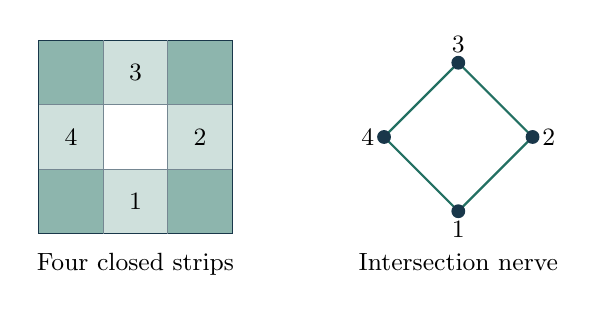
\begin{tikzpicture}[x=.82cm,y=.82cm,font=\small]
  \fill[accent!22] (0,0) rectangle (3,3);
  \fill[white] (1,1) rectangle (2,2);
  \foreach \x in {0,2} \foreach \y in {0,2}
    {\fill[accent!52] (\x,\y) rectangle ++(1,1);}
  \draw[ink] (0,0) rectangle (3,3);
  \draw[ink] (1,1) rectangle (2,2);
  \foreach \x in {1,2} {\draw[ink!60] (\x,0)--(\x,3);}
  \foreach \y in {1,2} {\draw[ink!60] (0,\y)--(3,\y);}
  \node at (1.5,.5) {1}; \node at (2.5,1.5) {2};
  \node at (1.5,2.5) {3}; \node at (.5,1.5) {4};
  \node[anchor=north] at (1.5,-.15) {Four closed strips};
  \begin{scope}[shift={(6.5,1.5)}]
    \coordinate (a) at (0,-1.15); \coordinate (b) at (1.15,0);
    \coordinate (c) at (0,1.15); \coordinate (d) at (-1.15,0);
    \draw[accent,thick] (a)--(b)--(c)--(d)--cycle;
    \foreach \pt in {a,b,c,d} {\fill[ink] (\pt) circle (2.5pt);}
    \node[below] at (a) {1}; \node[right] at (b) {2};
    \node[above] at (c) {3}; \node[left] at (d) {4};
    \node[anchor=north] at (0,-1.65) {Intersection nerve};
  \end{scope}
\end{tikzpicture}
\caption{Each darker square is an intersection of two strips and gives one edge of the nerve. There are no triple intersections. Both spaces have one independent loop.}
\label{fig:frame}
\end{figure}


\subsection{Arithmetic and Lean realization}

With $s$ cells and $m$ charts the incidence table has at most $s2^m$
ordinary columns. The added columns number at most $s$ or $2^m$.
A matrix can be packed as a list of bit masks of these bounded lengths.
For boxes, $s\le (4m)^d$ before removing cells outside the union.
Forming powers, testing local fillings, XOR summation, and sorting endpoints
by integer cross-products are primitive recursive in the full input,
including dimension. The outer correctness assertions quantify universally
over input codes. Inside a loop, assert by a Boolean test that all
previous columns obey their identity. For the power loop, test that all
nonzero entries lower the specified coordinate degree by at least the
current exponent. The indices in these tests range only over the two
explicit table sizes. In the telescoping identity one may compare each
matrix column, because equality of linear maps means equality of these
columns. Replacing bounded tests by their primitive recursive folds leaves
quantifier-free induction. A local test failure is an explicit alternative
of the total algorithm.

The Lean file \texttt{TopologyCase.lean} proves the nilpotent correction
identity for an abelian group of exponent two, including commutation of the
defect with $D$. Its bounded-lowering lemma derives nilpotence from a
strict decrease in the largest surviving opposite-coordinate degree. Its
common-coordinate bound proves the denominator estimate for $W$ after
clearing rational denominators. The executable \texttt{nerve.py} implements both local
constructions. To reach a full object derivation, represent a cell by a face
mask or a tuple of grid indices, implement the three arrays as bit matrices,
and instantiate in order the two-deletion cancellation, local-fill
induction, degree-lowering induction, and telescoping identity above.
Project the three block equations by bounded row and column indices before
composing the final maps. These are the remaining lemmas between the host
identity and the arithmetized chain equivalence.

\section{A uniform local solution at an integer resonance}
\label{sec:resonance}

At a regular singular point the two usual power-series solutions can collapse
into one. The Gauss hypergeometric report gives a finite recurrence in this
case and leaves a joint coefficient bound and convergence modulus for variable
resonance order to be supplied. We construct both, and determine exactly when
a logarithm is forced. The same construction applies to other scalar
second-order equations once one regular solution and a Wronskian density are
given. The source discussions occur in the resonance paragraphs of sections 5
and 10 of the repository's \texttt{hypergeometric\_ipra\_2026-11-16} report.

\subsection{Local integration with a variable pole order}
Use Gaussian rationals with $|x+iy|_1=|x|+|y|$. This norm is
submultiplicative. For a conditional object theorem the stated bounds on the input coefficient programs are supplied as iPRA derivations or retained as hypotheses. The coefficient of $z^n$ in a product is a sum over
$i+j=n$. A Laurent series here has an explicitly bounded finite principal
part. The arithmetic conclusions below are identities and error inequalities
for finite coefficient and value observations. The language of solution
germs describes the analytic interpretation of those conclusions.

Let $m$ be any natural number. Suppose two fixed PR procedures
(with numerical parameters) present $u=\sum u_nz^n$ and $g=\sum g_nz^n$,
with $u_0=g_0=1$ and a supplied integer $D\ge1$. Assume the arithmetical
hypotheses $|u_n|_1,|g_n|_1\le D^n$ for every $n$. In the Gauss
application below these inequalities follow from the recurrence. Define
\[
 w_0=1,\qquad w_n=-\sum_{i=1}^n u_iw_{n-i}\quad(n>0),\qquad
 h_n=\sum_{i+j+k=n}g_iw_jw_k,\qquad K=6D .
\]
Then $uw=1$ and $u^2h=g$ coefficient by coefficient. Inductively
$|w_n|_1\le(2D)^n$ follows by dividing the recurrence bound by $(2D)^n$ and using $\sum_{i=1}^n 2^{-i}\le1$. Each triple contributes at most
$(2D)^n$, and there are at most $3^n$ triples. Each triple is encoded
injectively by a word of $i$ zeros, $j$ ones and $k$ twos, including
the empty word. Thus $|h_n|_1\le K^n$.

Fix a nonzero Gaussian rational centre $z_*$ with $K|z_*|_1<1/4$.
Use rational samples $z$ with $K|z|_1\le1/4$ and
$|t|_1\le1/2$, where $t=(z-z_*)/z_*$. Set
\[
 L(z)=\sum_{j\ge1}(-1)^{j+1}t^j/j .
\]
Here $L(z_*)=0$ and $L'(z)=1/z$ because the derivative sums to
$1/[z_*(1+t)]$ by the finite geometric identity. The chart guard
guarantees $z\ne0$ since $t=-1$ fails it. Define
\begin{align}
 F(z)&=\sum_{n<m}\frac{h_n}{n-m}z^{n-m}+h_m L(z)+T(z), &
 T(z)&=\sum_{j\ge1}\frac{h_{m+j}}{j}z^j, \nonumber\\
 v(z)&=u(z)F(z), & F'(z)&=z^{-m-1}h(z). \label{eq:frob-pri}
\end{align}
The three terms of $F$ integrate the powers below $-1$, the power $-1$,
and the nonnegative powers. The finite sum is empty when $m=0$.

For $0\le d\le2$, omitting terms $j\ge J\ge 2$ in $T^{(d)}$
has error at most
\begin{equation}
                   4^{d+1}K^{m+d}2^{-J}.                   \label{eq:frob-tail}
\end{equation}
Indeed the coefficient magnitudes of $T$ are bounded by $K^{m+j}$.
The $j$th differentiated term on the chart is bounded by
$4^d K^{m+d}j^d4^{-j}$. For $j\ge2$, $j^d\le2^{j+1}$, by checking
$j=2,3$ and using $(j+1)^2\le2j^2$ for $j\ge3$. Sum the geometric
majorant to obtain \eqref{eq:frob-tail}. The same estimate with $m=0$
applies to $u,w,g,h$. For error $2^{-p}$ take
$J=2+p+4^{d+1}K^{m+d}$ since $C\le2^C$ for integral $C\ge1$.
The log tail is at most $2^{1-J}$ and its first two derivatives are the
rational functions $1/z,-1/z^2$.

Derivative assertions can themselves be read as finite remainder inequalities.
For a polynomial partial sum of a series with $|a_j|_1\le AK^j$, subtract
its value and linear term at $z$. By the binomial theorem the remainder at
$z+s$ has norm at most
\[
 |s|_1^2 AK^2\sum_{j\ge2}\binom j2 2^{-(j-2)}
 =8AK^2 |s|_1^2\qquad (K(|z|_1+|s|_1)\le1/2).
\]
For finite sums the bound $8$ follows by multiplying three finite geometric
sums of ratio $1/2$. Their triple coefficients are $\binom j2$ at
degree $j-2$ up to the truncation. For the derivative polynomial the
remainder is at most $48AK^3|s|_1^2$ by
$j\binom{j-1}{2}=3\binom j3$ and four geometric sums. Applying
\eqref{eq:frob-tail} at the two observed points proves the derivative
identities to arbitrary precision. One may enlarge a boundary chart
slightly within the open disk of convergence, replacing $1/4$ by any
rational ratio strictly below one and using its geometric tail. For $L$
apply the same polynomial proof with $|t|_1+|s/z_*|_1\le3/4$.
In particular no theorem on differentiating a general infinite limit
is needed.

Individual cutoffs give a cutoff for $v$ and each derivative. Evaluate
negative powers at rational $z$ exactly. A magnitude bound for each series
is one plus the norm of its precision-zero approximation. Propagate bounds
for sums and products by the triangle and product inequalities. To request
precision $p$ at a sum request $p+1$ at both children. At a product with
operand bounds $A,B$ request $p+\lceil A+B+2\rceil$ at both children,
since the product error is at most $(A+B+1)\epsilon$ for input
errors at most $\epsilon\le1$. Apply this rule also to the product
formulas for $v'$ and $v''$. It accounts for small denominators from the
principal part.

\paragraph{Local reduction of order.}
Suppose $u$ satisfies $y''+P y'+Qy=0$ on the chart, and
$W=z^{-m-1}g$ satisfies $W'=-PW$. Then $v$ in
\eqref{eq:frob-pri} satisfies the same equation and
$uv'-u'v=u^2F'=W$. Indeed $(u^2F')'=-Pu^2F'$ gives
$u^2F''+(2uu'+Pu^2)F'=0$. Expand the equation for $uF$, use the
equation for $u$, and cancel the unit $u$. The inverse exists since $uw=1$.
Also $|u-1|_1,|g-1|_1\le1/23$ by $D|z|_1\le1/24$.
In particular the inverse Wronskian is $z^{m+1}/g$, where $1/g$ is
computed by the same inverse-prefix rule. At an ordinary centre where
$P,Q$ have convergent Taylor data, the two solutions span the Taylor-solution
germs. Solve the two initial-value equations using this inverse Wronskian.
The difference has zero constant and linear coefficients. At order $j$ the
equation determines its next coefficient by a convolution of earlier ones
divided by $(j+2)(j+1)$, so every coefficient vanishes. Recentring a convergent
series on a smaller disk uses the binomial expansion. At parent degree $j$
the sum of norms of all translated terms is at most
$|a_j|_1(|z_*|_1+|s|_1)^j$, giving a geometric bound for the reordered
tails. Rational negative powers are handled by the local geometric inverse.

A Laurent derivative has zero coefficient at $z^{-1}$ because only the
derivative of a constant could contribute. If a Laurent solution with
a finite pole had normalized Wronskian $W$ with $u$, its quotient by $u$
would have derivative $z^{-m-1}h$, whose residue is $h_m$. Conversely,
if $h_m=0$ the displayed formula gives such a Laurent solution. This
obstruction is an identity of formal Laurent coefficients at zero.
The chart gives the local analytic realization.

\subsection{The Gauss equation and its exact logarithmic coefficient}
Take $a,b\in\mathbb Q(i)$, $c=m+1$, and put
\[
 \mathcal L y=z(1-z)y''+[c-(a+b+1)z]y'-aby.
\]
Starting at $u_0=g_0=1$, compute
\[
 u_{n+1}=\frac{(n+a)(n+b)}{(n+1)(n+m+1)}u_n,\qquad
 g_{n+1}=\frac{n-q}{n+1}g_n,\qquad q=m-a-b .
\]
Comparison of coefficients gives $\mathcal L u=0$ and
$(1-z)g'=-qg$. Write $P=[c-(a+b+1)z]/[z(1-z)]$.
The logarithmic derivative of $z^{-m-1}g$ is
$-(m+1)/z-q/(1-z)=-P$. The integer
\[
 D=\left\lceil\max\{1,\max(1,|a|_1)\max(1,|b|_1),|q|_1\}\right\rceil
\]
works for both series since $n+|a|_1\le(n+1)\max(1,|a|_1)$,
and the same inequality holds for $b$ and $q$. Thus the two local
solutions have a single PR precision schedule uniform in $m,a,b$.

Write $(x)_m=\prod_{j<m}(x+j)$. The logarithm in $v$ has multiplier $h_m u$,
where
\begin{equation}
             h_m=\frac{(-1)^m(a-m)_m(b-m)_m}{(m!)^2}.        \label{eq:frob-res}
\end{equation}
For $m=0$ this gives $h_0=1$. For $m>0$ separate the logarithmic term and
write the Laurent part of $v$ as $z^{-m}\sum_{j\ge0}d_jz^j$. Its leading
coefficient is $d_0=-1/m$. The logarithmic source has no powers below
$z^{-1}$ since
\[
 \mathcal L(u L)=2(1-z)u'+[m/z-(a+b)]u .
\]
For $0\le j<m-1$ the coefficient of $z^{j-m}$ therefore gives
\[
 (j+1-m)(j+1)d_{j+1}=(j+a-m)(j+b-m)d_j.
\]
At $z^{-1}$ the multiplier of $d_m$ is zero and the remaining equality is
$m h_m=(a-1)(b-1)d_{m-1}$. Multiplying through the previous $m-1$ steps
gives \eqref{eq:frob-res} because the denominator product is
$(-1)^{m-1}((m-1)!)^2$, with the other two factors of $m$ from $d_0$ and
the last equation. This includes $m=1$ via the empty product.
Hence for $m>0$ a second Laurent solution exists exactly when
$a$ or $b$ belongs to $\{1,\dots,m\}$, a decidable condition over Gaussian
rationals. In the reverse implication for an arbitrary independent
meromorphic solution, its Wronskian divided by $W$ has derivative zero.
Coefficientwise only the constant survives, and independence makes the
constant nonzero (apartness in the analytic reading). Rescaling would
therefore give a normalized solution.

For $c=1-m$ the substitution $y=z^mY$ gives the Gauss equation for $Y$
with parameters $a+m,b+m,1+m$. The extra coefficient of $z^{-1}Y$
is $m(m-1+c)=0$, the derivative coefficient becomes
$c+2m-(a+b+2m+1)z$, and the constant is $-(a+m)(b+m)$.
Consequently the construction covers every integer $c$ at zero.
Replacing $z$ by $1-z$ changes $c$ to $a+b+1-c$ and gives the analogous
local basis at one whenever $c-a-b$ is integral. The constants matching a
solution from a distant base point and the global Schwarz mapping problem
remain separate questions.

\paragraph{A resonant example.}
For $a=b=1/2$, $m=2$ one has $u_1=1/12$, $g=1-z$, $h_0=1$,
$h_1=-7/6$, and $h_2=9/64$. Hence the normalized second solution is
\[
 v=u\left(-\frac1{2z^2}+\frac7{6z}
             +\frac9{64}L(z)+\sum_{j\ge1}h_{2+j}z^j/j\right).
\]
Here $D=1$, $K=6$ and $z_*=1/48$ satisfies the chart guard. For
$a=1,b=5/3,m=3$, the coefficient $h_3$ vanishes and the second solution
is meromorphic at the singular point.

\paragraph{Object derivation and Lean completion.}
Code the Gaussian-rational pairs with positive denominators and clear them at
comparisons. Compute $(u_i,g_i,w_i,h_i)_{i\le N}$ by appending to bounded
tables. A QF induction assertion is the Boolean fold checking the defining
identities and the bounds for every index in the current prefix. Apply
the same finite convolution calculation to these prefixes to obtain $uw=1$,
$u^2h=g$ and the differential identities, retaining the needed coefficients
(e.g.\ through $m+j+2$ for Laurent powers through $z^j$ and two derivatives).
For \eqref{eq:frob-res} maintain the cross-multiplied recurrence product
through a prefix of length at most $m-1$. For \eqref{eq:frob-tail} take
arbitrary finite endpoints $J\le M$, bound the finite sum through $M$ by
the displayed geometric quantity, then universally close in $M,J,p$.
Use the same finite-endpoint convention for products by bounding the partial
convolution tail at a strict radius by grouping triples by total degree,
using the bound $(6D)^j$ above. These inductions use integer equalities,
cross-multiplied inequalities or bounded Boolean checks. The universal input
bounds on the two coefficient families stay in the context of induction.

The accompanying \texttt{lean/Resonance.lean} implements the real-rational
coefficient tables and product formula, proves the size of the inverse table,
the order-zero coefficient, the bounded zero test for the product formula,
and a precision inequality, and kernel-checks the
two examples. For the object theorem first lift these definitions to pairs of
rational codes including the signed coefficients of the finite principal part.
Next derive the prefix estimates and identities just listed. Lastly use the
error circuits to construct the chart's first two derivative names. The
repository's \texttt{HypergeometricOdeFormal} contains the formal Wronskian
derivative identity, and \texttt{ComplexLogarithmName} constructs a local
logarithm name. The latter leaves the derivative law open. The finite
geometric identity and difference estimate above supply its mathematical
proof after identifying the two local power-series observations. A direct
implementation can use the displayed chart throughout. The supplied Lean
file covers finite lemmas and examples. The full object-language derivation
remains to be built. The independent exact tests in
\texttt{code/resonance.py} compare the convolution and product answers and
check the coefficients of the inhomogeneous Laurent recurrence.

\section{Formalization and reproducibility}
\label{sec:replay-guide}
\subsection{How the applications use the same interface}
For each port one must give a formula, the scope of its parameters and the proof or program that supplies it. The following three examples show where this changes a mathematical conclusion.
\begin{itemize}
\item In the nerve argument each nonempty overlap $I$ has a label $H_I$ asserting that its displayed augmented chain contraction satisfies $\partial h+h\partial=1$. A checked table of fillings supplies $H_I$, and the box formula supplies it directly on rectangular instances. With $s$ and $m$ as in Section~\ref{sec:nerve-case}, all equalities of columns admit bounded tests. The general contraction algorithm uses $\bigwedge_I H_I$ once for the vertical elimination. The horizontal elimination has an independent producer using the least containing chart. Together they produce the two inverse chain maps. Since the output includes the homotopy matrices, a downstream user can check their identities directly without retaining all the original local witnesses.
\item In a tower the target at a chosen depth $j$ is the pair of finite checks that the constructed element has the correct image and that it projects to the initial one. A row extends a prefix by one level. The port at that level compares just two images, computable by search in finite fibers. Induction is on the reflected prefix check while the premise that the image comparison holds at every level remains in the context. The obstruction based on delayed halting explains why a variable tower cannot silently acquire this premise. For a single requested finite horizon it suffices to supply the comparisons reached by that horizon.
\item In the Gauss calculation a query $(m,a,b,J)$ requests a finite coefficient list. Product, inverse and integration each consume finite prefixes with explicit lengths. For $m>0$ the label asserting the existence of a second meromorphic solution has two sufficient input tests, $a\in\{1,\ldots,m\}$ and $b\in\{1,\ldots,m\}$. The exact residue computation proves that these are also semantically exhaustive for the presented coefficients. This extra necessity is a mathematical theorem. Saturating a rule table alone proves completeness only for proofs assembled from its rows.
\end{itemize}

\subsection{What Lean checked}
\small
\begin{tabular}{@{}p{.245\linewidth}p{.695\linewidth}@{}}
\toprule
File & Endpoint and scope\\
\midrule
\path{CyclicReplay.lean} & \texttt{stabilized} and \texttt{all\_heights} prove the finite saturation bound and completeness for the executable table. The support theorem also characterizes every successful supply by containment of an inclusion-minimal one. \texttt{replay} returns $\Gamma\vdash A_v$ for each marked label given local derivations and port proofs. \texttt{two\_supports} produces the object-language disjunctive condition for the displayed cyclic example.\\[4pt]
\path{AtlasCase.lean} & \texttt{envelope\_transfer} and \texttt{transfer\_guard} verify the max--min estimate and the chart selected from an approximation. The vertex algorithm is proved in Section~\ref{sec:atlas}.\\[4pt]
\path{SheafCase.lean} & Principal-neighborhood gluing, \texttt{along\_extend} and \texttt{extend\_along} prove the reflector's inverse laws for presheaves in Lean. The finite mask and mixed-radix implementations are described in Section~\ref{sec:categorycases}.\\[4pt]
\path{CategoryCase.lean} & \texttt{local\_iff\_stable}, the bounded lift and the coherent walk for an inverse tower with specified projection laws. The universal image-stability result is a semantic Lean theorem.\\[4pt]
\path{TopologyCase.lean} & The nilpotent correction producing a contraction, a degree-lowering lemma and the positive denominator estimate for the box homotopy. Matrices, subdivisions and maps on regular names are developed in Section~\ref{sec:nerve-case}.\\[4pt]
\path{Resonance.lean} & Finite rational coefficient computation, the zero criterion for the closed rational product, a cutoff inequality, and two evaluated examples. Section~\ref{sec:resonance} proves the coefficient formula and Gaussian-rational analytic estimates.\\
\bottomrule
\end{tabular}
\normalsize

\medskip
The Lean run used version 4.32.0. We freshly compiled \texttt{Syntax}, \texttt{Deduction} and \texttt{PR} from the pinned revision. Their Git blob identifiers are recorded with the replay instructions. Mathlib was at the repository's pinned revision. The reported Lean dependencies of \texttt{replay} and \texttt{two\_supports} are \texttt{propext}, \texttt{Classical.choice} and \texttt{Quot.sound}. These concern Lean's construction of a proof whose type is \texttt{Prf PRAAx}. Its object-level axioms are the constructors of \texttt{PRAAx}. The semantic tower equivalence prints no axiom dependencies. The individual application theorems do not yet have end-to-end \texttt{Prf PRAAx} files.

\subsection{Completing the object-language derivations}
Use \texttt{PR k} for the programs, \texttt{PTm n} for terms with $n$ free variables, and \texttt{Fm PTm n} for formulas. Construct a program with zero, successor, projections, composition and primitive recursion, bundling simultaneous state in a pair or a list. After replacing displays involving rational numbers by integer-part pairs and positive denominators, the governing target for a total algorithm $t$ with precondition $D$ is
\[
 []\vdash \forall\vec x\,\big(D(\vec x)\longrightarrow
                   V(\vec x,t(\vec x))\big).
\]
Open versions in a context can then be specialized by substitution. A valid unsupplied assumption is retained in $D$. A computed output carries its defining recurrence and correctness theorem. Source links below use repository paths at the pinned revision.

\begin{enumerate}
\item \emph{Reflection.} Build each bounded input and invariant as a \texttt{BFm n} and apply its reflection and induction lemmas. Use \texttt{mu} only with a proved existence below its cap, or treat the sentinel as failure. This handles zero-size fibers, missing parents and singular determinant candidates. \repo{Derivations/Lean/IPRADerivations/Foundations/BoundedSyntax.lean}{Bounded syntax} and \repo{Derivations/Lean/IPRADerivations/Foundations/BoundedSelection.lean}{bounded selection}.
\item \emph{Numerical cyclic tables.} Pack $N,b$ and the rows into the parameter $x$. Define the new bit for $v$ as its old bit or a bounded OR over matching heads whose two mask tests hold. Bounds $2^N$ and $2^b$ suffice for valid masks. Derive coordinate monotonicity from conjunction monotonicity and supply all-one caps to \texttt{closure\_prefixed}. Alternatively use the rank-or-flat proof of Theorem~\ref{th:closure} on the count of marked bits. Define first-entry rank as the least $j\le N$ with membership, storing a separate membership flag for failure. A second bounded scan returns the first row justified at stage $j-1$. Prove its two conditions from the recursion, then invoke the reflected invariant of Section~\ref{sec:rules}. Run the same operator with ports removed singly to compute the minimality test. This implements the internal input-uniform form corresponding to the external Lean replay. \repo{Derivations/Lean/IPRADerivations/Foundations/DemandClosure.lean}{Demand closure} and \repo{Derivations/Lean/IPRADerivations/Foundations/FrontierSoundness.lean}{rank induction}.
\item \emph{Polyhedral charts.} Encode a hyperplane as its packed row of integer coefficients, a candidate as a tuple of $d$ indices, and a rational point as $d$ numerator/denominator pairs. Use signed permutation enumeration for the determinant. Prove its alternating and column expansion laws by pairing permutation terms, then the rational linear-solve lemma by multiplication with the adjugate. Enumerate all minors to obtain rank and null vectors, run the $d$-step algorithm with invariant in Section~\ref{sec:atlas}, and use its output to prove the returned minimum against an arbitrary rational point. Finish with the displayed Lipschitz estimate at the clipped rational approximant.
\item \emph{Category and topology.} The finite sheaf inverse equations reduce to comparisons over the coordinates of minimal opens. Lift the coherent-tower algorithm by distinguishing the code for a level from the external PR symbol for projection. For the maps of boxes first prove exact rational simplex interpolation and face agreement, then derive pointwise estimates for regular names from the computed bounds. A name of a point of a polyhedron may use rational approximants in that polyhedron as its presentation. Equivalently one can select nearby grid-simplex points by rational finite approximations with a supplied proximity bound. The first presentation suffices here. For the chain part all matrix columns are bounded masks, including the block identities extracting the homotopies. See the \repo{Derivations/Lean/IPRADerivations/Foundations/CoherentTower.lean}{tower backend} and the \repo{docs/proofs/topology/ipra_topology_framework_2026-11-15/paper/sections/12_limits.tex}{topological limitations report}.
\item \emph{Analysis.} First prove the finite polynomial and Laurent identities on exact Gaussian rationals. Next prove the inequalities for arbitrary finite tails, with both endpoints free. Finally construct the three observation programs for value, first derivative and second derivative. Their precision budgets in Section~\ref{sec:resonance} can be composed by PR recursion. A global coefficient bound in the generic lemma is a hypothesis on its two fixed programs. The Gauss instance proves it by the two first-order recurrences. The disc-center and branch datum are explicit inputs. \repo{docs/proofs/analysis/hypergeometric_ipra_2026-11-16/sections/05_ode.tex}{Gauss ODE packet}, \repo{docs/proofs/analysis/hypergeometric_ipra_2026-11-16/sections/10_continuation.tex}{continuation scope} and \repo{Derivations/Lean/IPRADerivations/Analysis/HypergeometricOdeFormal.lean}{formal ODE derivations}.
\end{enumerate}

\paragraph{Further research questions.}
Can the finite acyclic-overlap construction be lifted to integral chain equivalences using a similar size bound on the coefficients of the produced contractions? For the resonant Gauss equation, can a finite chain of certified charts yield connection matrices with uniform precision bounds as a path passes between a resonant chart and an ordinary one? Can the object-language graph compiler accept and check one ranked table of outputs with quantified certificate fields, while identifying exactly the fields that need bounded witnesses? Proposition~\ref{p:path} imposes a concrete test on any such extension. A successful answer must specify which invariant supports input-length induction.


\subsection{Replaying the examples}
From the extracted archive run \texttt{python3 verify.py}. It executes six programs with exact integer and rational operations. With the specified ProveIt checkout and its prebuilt providers, \texttt{python3 verify.py {-}{-}proveit /path/to/ProveIt} also elaborates all six Lean modules. The archive README records the inputs and the build commands. The transcript in \path{verification/results.txt} includes the axiom reports.

\begin{center}\small
\begin{tabular}{@{}p{.24\linewidth}p{.69\linewidth}@{}}
\toprule
Computation & Independent check or observed value\\
\midrule
Rule tables & For 21,956 table/supply pairs, intersecting all closed masks and eliminating one feedback variable both reproduce the iterated mask. All minimal supplies were checked at both output labels.\\[3pt]
Presheaves and towers & 94 morphism pairs passed both inverse checks. Of 7,680 proposed rates on 64 finite towers, 3,792 passed the comparison. Their constructed walks passed 153,744 edge tests.\\[3pt]
Covers & The square chart margin is $1/6$. The test segment clears the two punctures by exactly $1/3$. The rectangle frame and cube boundary give Betti vectors $(1,1,0)$ and $(1,0,1)$ through degree two.\\[3pt]
Homotopies & The rational homotopies were evaluated at five times on 96 points of the frame and 189 points in two nerves. A disconnected intersection was rejected by the chain test.\\[3pt]
Resonance & The inverse-series expression and the finite product agree on 392 Gaussian-rational parameter triples. The Laurent recurrence gives the log multiplier $9/64$ when $a=b=1/2$ and $c=3$.\\
\bottomrule
\end{tabular}
\end{center}
\begin{thebibliography}{9}
\bibitem{proveit} V. Reshetnikov et al. \emph{ProveIt, Primitive Recursive Arithmetic}. Source snapshot and attached status reports. \repo{README.md}{Repository index}.
\bibitem{green} T. J. Green, G. Karvounarakis and V. Tannen. \emph{Provenance semirings}. PODS 2007, 31--40. \href{https://doi.org/10.1145/1265530.1265535}{doi:10.1145/1265530.1265535}.
\bibitem{dlmf} A. B. Olde Daalhuis. Hypergeometric Function, \S15.10, in \emph{NIST Digital Library of Mathematical Functions}. Classical resonant solution formulas for comparison. \url{https://dlmf.nist.gov/15.10}.
\end{thebibliography}

\end{document}
